% =============================================================================
% File:  sample_slides.tex --  Example of the use of the Falkor Beamer theme
% Author(s): Sebastien Varrette <Sebastien.Varrette@uni.lu>
% Time-stamp: <Mar 2014-04-29 16:06 svarrette>
% 
% Copyright (c) 2012 Sebastien Varrette <Sebastien.Varrette@uni.lu>
% .             http://varrette.gforge.uni.lu
% 
% For more information:
% - LaTeX: http://www.latex-project.org/
% - Beamer: https://bitbucket.org/rivanvx/beamer/
% - LaTeX symbol list:
% http://www.ctan.org/tex-archive/info/symbols/comprehensive/symbols-a4.pdf
% 
% Latest version of these files can be found on Github:
% 

% =============================================================================
\documentclass{beamer}
% \documentclass[draft]{beamer}
\usepackage{_style}
\usepackage{__config}

% The key part to use my theme
\usetheme{Falkor}

% Not integrated in my theme as not everybody wants that
\AtBeginSection[]
{
  \frame{
    \frametitle{Summary}%
    {\scriptsize\tableofcontents[currentsection]}
  }
}

%%%%%%%%%%%%%%%%%%%%%%%%%%%% Header %%%%%%%%%%%%%%%%%%%%%%%%%%%%%%
\title{\EventName}
\subtitle{\TPindex: \TPtitle}

\author{\authors}
\institute[UL]{
  University of Luxembourg, Luxembourg
}

% Mandatory to define a logo - otherwise compilation will fail in an unobvious
% manner.
\pgfdeclareimage[height=0.8cm]{logo}{images/logo_UL.pdf}
\logo{\pgfuseimage{logo}}
\date{}

%%%%%%%%%%%%%%%%%%%%%%%%%%%%%% Body %%%%%%%%%%%%%%%%%%%%%%%%%%%%%%%
\begin{document}

\begin{frame}
    \vspace{2.5em}
    \titlepage
\end{frame}

% .......
\frame{
  \begin{center}
      \textbf{Latest versions available on
        \href{https://github.com/ULHPC/}{Github}}:
      \vfill
      \begin{description}
        \item[UL HPC tutorials:] \hfill
          \myurl{https://github.com/ULHPC/tutorials}
        \item[UL HPC School:] \hfill
          \myurl{http://hpc.uni.lu/hpc-school/}
        \item[\TPindex tutorial sources:] \hfill
          \myurl{\TPghurl}
      \end{description}
  \end{center}
}

% ......
\frame{
  \frametitle{Summary}
  {\scriptsize
    \tableofcontents
  }
}

% ===============================================
\section{Objectives}

% ............
\frame{

  \frametitle{Objectives of the PS}

  \begin{itemize}
    \item Run sequential, parametric programs on the clusters
    \item Learn how-to use our set of launcher scripts
    \item Submit jobs, and use the cluster monitoring tools 
    \begin{itemize}
         \itemhook drawgantt
         \itemhook monika
         \itemhook ganglia
    \end{itemize}
  \end{itemize}

  \begin{exampleblock}{Read the full subject of this PS here}
      \begin{itemize}
        \item http://git.io/5cYmPw
      \end{itemize}
  \end{exampleblock}

}


% ===============================================
\section{Pre-requisites}

% Example of prompt usage
% .......
\begin{frame}[fragile]
    \frametitle{MPI tasks: getting started}
    \begin{enumerate}
      \item Connect to the cluster(s)\\
        \begin{cmdline}
            \cmdlinenode{ssh chaos-cluster}\\
            \cmdlinenode{ssh gaia-cluster}
        \end{cmdline}

      \item Transfer files
        \begin{cmdline}
            \cmdlinenode{rsync -avz directory chaos-cluster:}
        \end{cmdline}

      \item  Submit jobs:
        \begin{cmdline}
            \cmdlinenode{oarsub -I}\\
            \cmdlinenode{oarsub ./program}\\
        \end{cmdline}
	\end{enumerate}
	
    \begin{exampleblock}{Follow this part: "Connect the the cluster and set-up the environment for this tutorial"}
      \begin{itemize}
        \item http://git.io/5cYmPw
      \end{itemize}
    \end{exampleblock}	
	
\end{frame}





\section{Exercise 1: parametric execution of Gromacs}

% .......
\frame{
  \frametitle{Gromacs}

  \textbf{GROMACS}: GROningen MAchine for Chemical Simulations \\                                                                                                     
  \hfill \scriptsize{versatile package for molecular dynamics, primarily designed for biochemical molecules}
  \\ \hfill \\
  \begin{itemize}
    \item very large codebase: 1.836.917 SLOC
    \item many applications in the package, several parallelization modes
    \item \textbf{mdrun}: computational chemistry engine, performing:\\
      {
      \scriptsize
      $ \hookrightarrow $ molecular dynamics simulations \\
      $ \hookrightarrow $ Brownian Dynamics, Langevin Dynamics \\
      $ \hookrightarrow $ Conjugate Gradient \\
      $ \hookrightarrow $ L-BFGS \\
      $ \hookrightarrow $ Steepest Descents energy minimization \\
      $ \hookrightarrow $ Normal Mode Analysis \\
      }
    \item \textbf{mdrun} - parallelized using MPI, OpenMP, pthreads and with support for GPU acceleration
  \end{itemize}
}

% .......
\frame{
  \frametitle{Exercise 1: parametric execution}
    
  \begin{exampleblock}{2 approaches}
      \begin{itemize}
        \item Sequential (loop)
		\item Parallized (with GNU parallel)
      \end{itemize}
  \end{exampleblock}
\vspace{-1em}
  \center 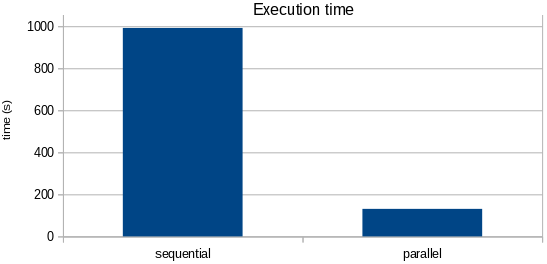
\includegraphics[scale=0.6]{images_custom/ps2-1-comparison}


}



\section{Exercise 2: Watermarking images in Python}

% .......
\frame{
  \frametitle{Task: apply a watermark to a given set of pictures}

      \begin{itemize}
        \item Simple Python script
        \item Generic parallel launcher
		\item Distribute the work on several nodes
      \end{itemize}

  \center 
\includegraphics[scale=0.20]{images_custom/ps2-2-copyright}

}

\frame{
 
  \center 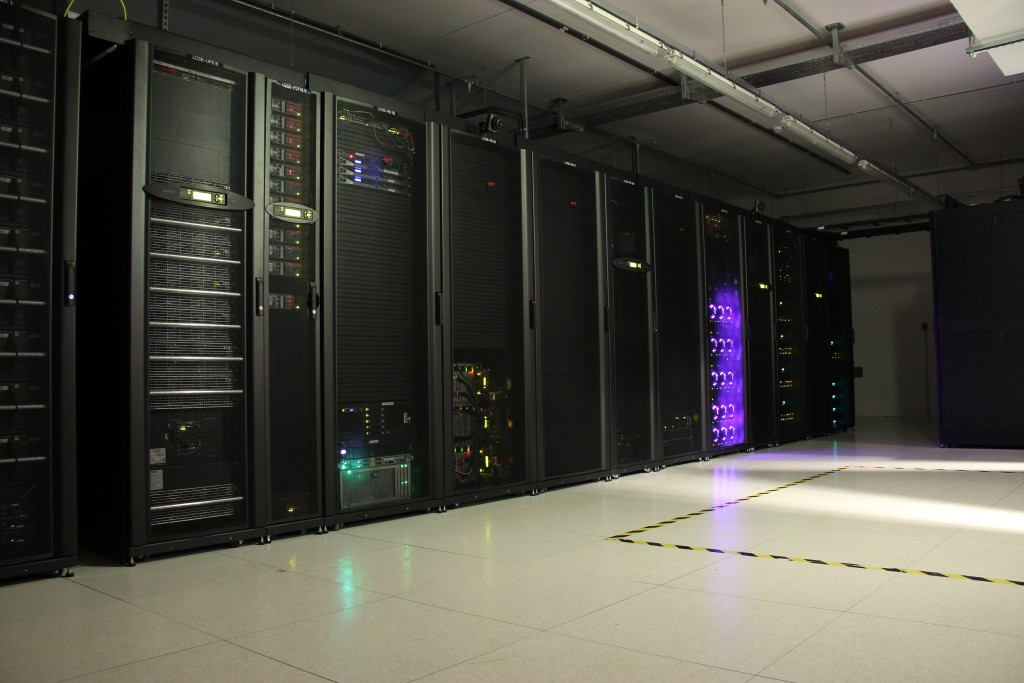
\includegraphics[scale=0.37]{images_custom/ps2-2-IMG_3155}

}

\frame{
 
  \center 
\includegraphics[scale=0.37]{images_custom/ps2-2-IMG_3155-watermarked}

}

\section{Exercise 3: Advanced use case, using a Java program: "JCell"}

% .......
\frame{
  \frametitle{Subject}

      \begin{itemize}
        \item \textbf{JCell}: a Java framework for working with genetic algorithms
        \item Example: Generational algorithm for the Combinatorial ECC problem
        \item Test the variations of these parameters: \textit{Mutation probability} and \textit{Crossover probability}
      \end{itemize}

}

\frame{

  \center 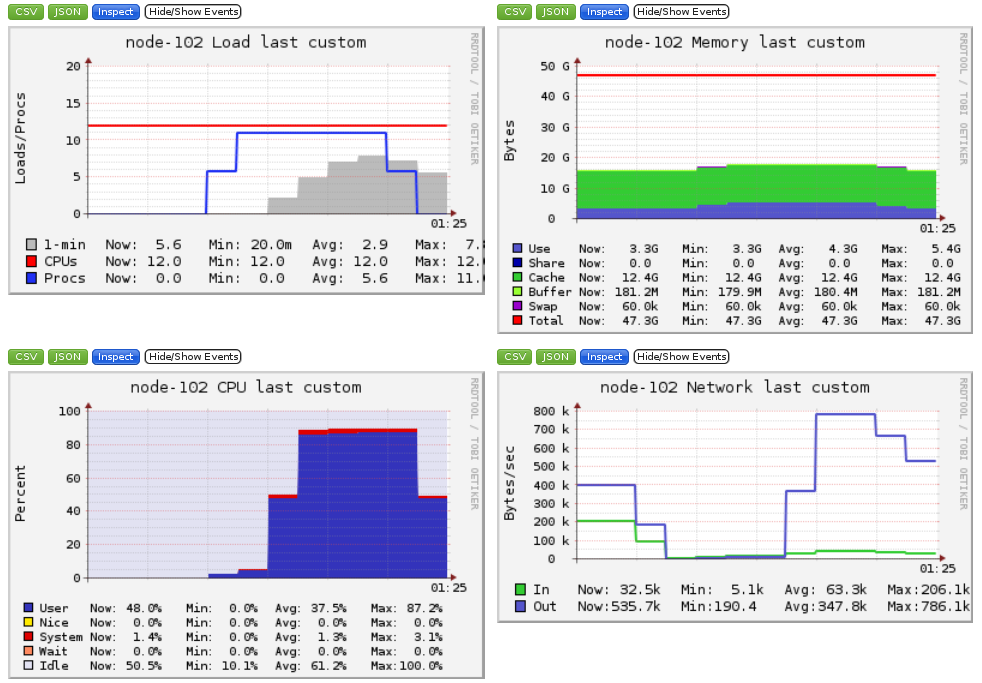
\includegraphics[scale=0.37]{images_custom/ps2-3-ganglia}

}

\section{Conclusion}

% ............
\begin{frame}
    \frametitle{Conclusion}

    \begin{itemize}
      \item We have covered the most common workflow: \textbf{parametric jobs}
      \item Our launchers can be improved!
    \end{itemize}

    \begin{block}{Perspectives}
        \begin{itemize}
          \item Checkpoint/Restart mechanism
          \item Best effort jobs
          \item OAR array jobs
        \end{itemize}
    \end{block}


\end{frame}

\section*{Thank you for your attention...}
\frame{
  \frametitle{Questions?}
  \begin{center}
      
\includegraphics[scale=0.2]{question.jpg}
  \end{center}

  {\tiny
    \tableofcontents

  }
}

\end{document}

% ~~~~~~~~~~~~~~~~~~~~~~~~~~~~~~~~~~~~~~~~~~~~~~~~~~~~~~~~~~~~~~~~
% eof
% 
% Local Variables:
% mode: latex
% mode: flyspell
% mode: auto-fill
% fill-column: 80
% End:
